\chapter{State of the Art}

In this chapter we will explain the current state of computer graphics its latest advances and how ray tracing fits into it. We will also be looking at the technologies being used in both research and industry. 

% Explain basis of ray tracing and how it compares against rasterization
\section{Rendering Techniques}
The field of computer graphics seeks to generate images with the aid of computers. Nowadays this is a core component of photography, film production and videogames among others. This task is commonly refered to as \textit{rendering}. Throughout the years there have appeared many rendering techniques, of which the main ones being used currently are Rasterization and Ray Tracing.

\subsection{Rasterization}
Rasterization is the process of taking an image described as vector graphics and converting it into a series of pixels which, when displayed together, recreate the image that was represented with vector shapes. This image can then be displayed in a monitor, stored as a bit map and so on.

In figure \ref{rasterization-triangle-image}, from \cite{ScratchPixel} we see the principle of this process. After transforming the geometry (in this case a triangle) to screen space, we check if each pixel in the image overlaps said geometry.

\begin{figure}[hbt!]
    \centering
    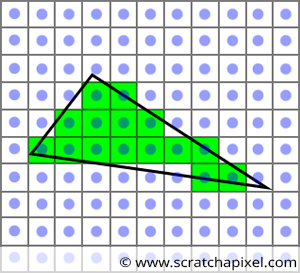
\includegraphics[width=1.0\textwidth]{figuras/rasterization-triangle1.png}
    \caption{}
    \label{rasterization-triangle-image}
\end{figure}
When compared to other techniques for rendering 3D models, such as ray tracing, rasterization is extremely fast. This gives it a prevalent usage in real time 3D engines. We must take into account that the process of rasterization is only responsible for mapping the scene geometry to pixels, and does not compute the color of such pixels. This color is assigned by a Pixel (or Fragment) Shader, which is completely programmable in modern GPUs. This shader may take into account physical processes like light position, or a purely artistic approach. There is no motivation in modifying the rasterization techniques at render time. Therefore, the rest of the process of rasterizing a 3D model into screen space (a 2D plane for displaying said graphics) is often performed by non-programmable hardware with a fixed function within the graphics pipeline. This method allows for high efficiency.

\subsection{Ray Tracing}
The other prevalent technique for drawing 3D graphics, and the main focus of this work, is ray tracing.

This technique models light transport for generating digital images. It does this tracing a path from an imaginary eye through each pixel in a virtual screen and calculating the color of the object visible through it. Each ray is tested for intersection with some subset of the objects in the scene. Once identified the object, it estimates the incoming light at the intersection point and read the material properties of the object to calculate the final color of the pixel.

Although counter intuitive, sending rays \textit{from} the camera towards the scene is many orders of magnitude more efficient than doing it the other way around. This is due to the vast majority of rays coming from a light source not reaching the viewer's eye, thus saving a lot of computation in paths that are never recorded. We take the shortcut of assuming that a given ray intersects the view frame. After a certain number of reflections or distance traveled by a ray without intersecting anything, that ray ceases to travel and the pixel's value is updated. Figure \ref{rt-overview-image} shows an overview of this algorithm extracted from the Wikimedia \cite{WikimediaRT}.


\begin{figure}[hbt!]
    \centering
    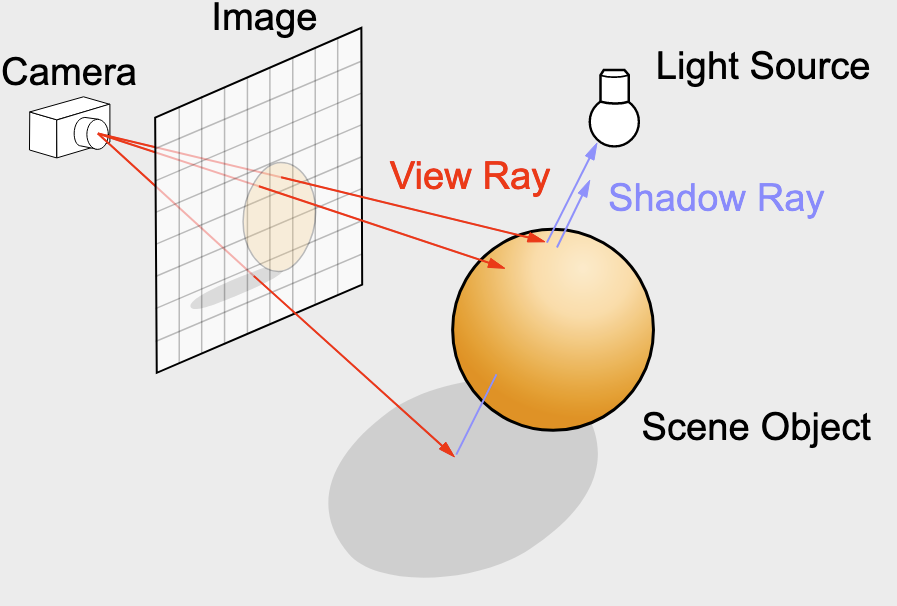
\includegraphics[width=1.0\textwidth]{figuras/RT-Diagram.png}
    \caption{Overview of the ray tracing algorithm with spheres as our only geometry and a single light source.}
    \label{rt-overview-image}
\end{figure}

Compared to rasterizing, all the techniques based in ray tracing are generally slower yet provide higher fidelity results than it's counterpart. This made it so that originally it was applied in tasks that could tolerate a relatively long render time, such as film production or still image generation. Applications where rendering speed is critical, like videogames, were less suited for these algorithms. However, since 2018, real time ray tracing has become more feasible thanks to hardware acceleration becoming standard in commercial graphics cards.

\subsubsection{Mathematical foundation}
We will now look at the mathematical definition of ray tracing applied to a rectangular viewport, which is the focus area of this work.

Our inputs are:
\begin{itemize}
  \item[*]{An eye position $E \in \mathbb{R}^3$}
  \item[*]{A target position $T \in \mathbb{R}^3$}
  \item[*]{A field of view $\theta \in [0, \pi]$. For humans, we can assume it's about 90 degrees ($\approx \frac{\pi}{2} radians $)}
  \item[*]{The number of square pixels in the vertical and horizontal directions in the viewport $m, k \in \mathbb{N}$}
  \item[*]{The actual number of pixels $i, j \in \mathbb{N}, 1 \leq i \leq k \land 1 \leq j \leq m$}
  \item[*]{A vertical vector that indicates the up and down direction $\overrightarrow{v} \in \mathbb{R}^3$. Usually $\overrightarrow{v} = [0, 1, 0]$ (the roll component determines the viewport's rotation around it's center $C$, where the axis is the $ET$ rotation).}
\end{itemize}

We can see an illustration of these components in figure \ref{RaysViewportSchema}, extracted from the Ray Tracing Wikipedia article \cite{WikipediaRT}.

\begin{figure}[hbt!]
    \centering
    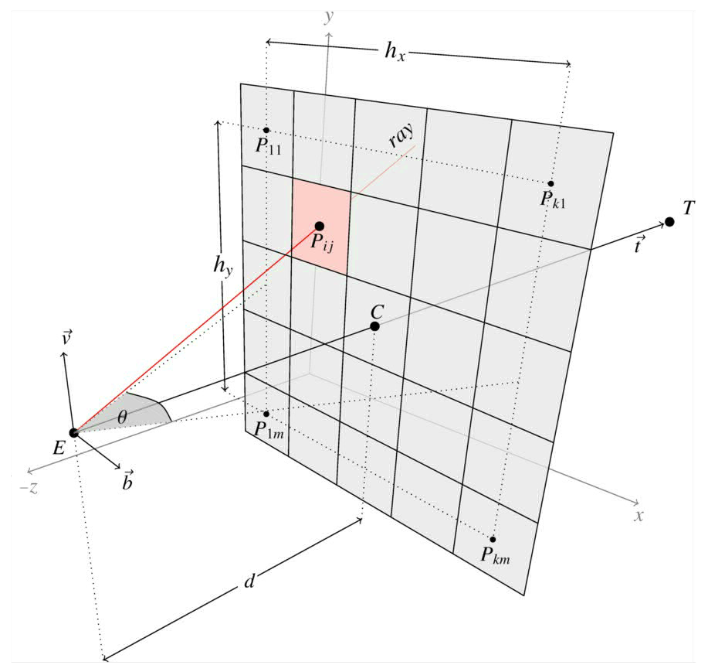
\includegraphics[width=1.0\textwidth]{figuras/RaysViewportSchema.png}
    \caption{Ray tracing schema with all the input components.}
    \label{RaysViewportSchema}
\end{figure}

With these inputs, our goal is to find the position of the center of each viewport pixel $P_{ij}$. This will allow us to find the line going from the eye $E$ through that pixel, and describe that ray by the point $E$ and the vector $\overrightarrow{R}_{ij} = P_{ij} - E$ (or its normalization $\overrightarrow{r}_{ij}$).

We start by finding the coordinates of the bottom left viewport pixel $P_{1m}$, and the subsequent ones by shifting along the directions paralell to the viewport (vectors $\overrightarrow{b}_{n}$ and $\overrightarrow{v}_{n}$), multiplied by the pixel size. The equations below include a distance $d$ between the eye $E$ and the viewport. This value will be reduced when normalizing the rays $\overrightarrow{r}_{ij}$, and as such can be interpreted as $d=1$ and removed from the calculations.

As a pre-calculation we normalize the vectors $\overrightarrow{t}$, $\overrightarrow{b}$ and $\overrightarrow{v}$, shown in figure \ref{RaysViewportSchema}, which are paralell to the viewport. This process is explained in equations \ref{eq-t-b}, \ref{eq-tn-bn} and \ref{eq-vn}.

\begin{equation}
  \overrightarrow{t} = T - E
  \text{,}
  \overrightarrow{b} = \overrightarrow{t} \times \overrightarrow{v}
  \label{eq-t-b}
\end{equation}

\begin{equation}
  \overrightarrow{t}_{n} = \frac{\overrightarrow{t}}{\left\Vert \overrightarrow{t} \right\Vert}
  \text{,}
  \overrightarrow{b}_{n} = \frac{\overrightarrow{b}}{\left\Vert \overrightarrow{b} \right\Vert}
  \label{eq-tn-bn}
\end{equation}

\begin{equation}
  \overrightarrow{v}_{n} = \overrightarrow{t}_{n} \times \overrightarrow{b}_{n}
  \label{eq-vn}
\end{equation}

Note that the viewport center is $C = E + \overrightarrow{t}_{n}d$.

We then calculate the viewport sizes $h_x$ and $h_y$, divided by $2$ including the inverse aspect ratio $\frac{m-1}{k-1}$. This is done in equation \ref{eq-g}.

\begin{equation}
  g_x = \frac{h_x}{2} = d * tan \frac{\theta}{2}
  \text{,}
  g_y = \frac{h_y}{2} = g_x \frac{m-1}{k-1}
  \label{eq-g}
\end{equation}

Next, we calculate the vectors used for shifting to the next pixel, $q_x$ and $q_y$, along the directions paralell to the viewport $\overrightarrow{b}$ and $\overrightarrow{v}$, from the bottom left pixel $p_{1m}$. This is shown in equations \ref{eq-q} and \ref{eq-p}.

\begin{equation}
  \overrightarrow{q}_x = \frac{2g_x}{k-1} \overrightarrow{b}_n
  \text{,}
  \overrightarrow{q}_y = \frac{2g_y}{m-1} \overrightarrow{v}_n
  \label{eq-q}
\end{equation}

\begin{equation}
  \overrightarrow{p}_{1m} = \overrightarrow{t}_n d - g_x \overrightarrow{b}_n - g_y \overrightarrow{v}_n
  \label{eq-p}
\end{equation}

If we consider $P_{ij} = E + \overrightarrow{p}_{ij}$ and the ray $\overrightarrow{R}_{ij} = P_{ij} - E = \overrightarrow{p}_{ij}$, we get the normalized rays in equation \ref{eq-r}.

\begin{equation}
  \overrightarrow{p}_{ij} = \overrightarrow{p}_{1m} + \overrightarrow{q}_x(i - 1) + \overrightarrow{q}_y(j - 1)
  \text{,}
  \overrightarrow{r}_{ij} = \frac{\overrightarrow{R}_{ij}}{\left\Vert \overrightarrow{R}_{ij} \right\Vert} = \frac{\overrightarrow{p}_{ij}}{\left\Vert \overrightarrow{p}_{ij} \right\Vert}
  \label{eq-r}
\end{equation}

% Introduce Vulkan and OptiX: main features, current real world usage, API organization, etc.
\section{Ray Tracing Technologies}
